\documentclass[xetex,mathserif,serif]{beamer}
\usepackage{polyglossia}
\setdefaultlanguage[babelshorthands=true]{russian}
\usepackage{minted}
\usepackage{tabu}

\useoutertheme{infolines}

\usepackage{fontspec}
\setmainfont{FreeSans}
\newfontfamily{\russianfonttt}{FreeSans}

\usepackage{forest}
\usetikzlibrary{arrows}

\definecolor{links}{HTML}{2A1B81}
\hypersetup{colorlinks,linkcolor=,urlcolor=links}

\tabulinesep=0.7mm

\title{Стек и куча}
\author[Юрий Литвинов]{Юрий Литвинов \newline \textcolor{gray}{\small\texttt{yurii.litvinov@gmail.com}}}

\date{08.09.2020}

\begin{document}
    
    \frame{\titlepage}
    
    \begin{frame}
        \frametitle{Указатели и куча}
        \begin{center}
            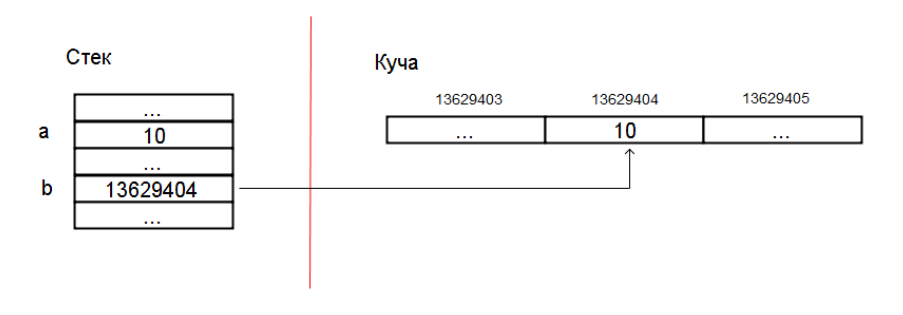
\includegraphics[width=0.8\textwidth]{pointers.png}
        \end{center}
    \end{frame}

\end{document}

